
\documentclass[border=8pt, multi, tikz]{standalone} 
\usepackage{import}
\subimport{../layers/}{init}
\usetikzlibrary{positioning}
\usetikzlibrary{3d} %for including external image 

\def\ConvColor{rgb:yellow,5;red,2.5;white,5}
\def\ConvReluColor{rgb:yellow,5;red,5;white,5}
\def\PoolColor{rgb:red,1;black,0.3}
\def\UnpoolColor{rgb:blue,2;green,1;black,0.3}
\def\FcColor{rgb:blue,5;red,2.5;white,5}
\def\FcReluColor{rgb:blue,5;red,5;white,4}
\def\SoftmaxColor{rgb:magenta,5;black,7}   

\newcommand{\copymidarrow}{\tikz \draw[-Stealth,line width=0.8mm,draw={rgb:blue,4;red,1;green,1;black,3}] (-0.3,0) -- ++(0.3,0);}

\begin{document}
\begin{tikzpicture}
\tikzstyle{connection}=[ultra thick,every node/.style={sloped,allow upside down},draw=\edgecolor,opacity=0.7]
\tikzstyle{copyconnection}=[ultra thick,every node/.style={sloped,allow upside down},draw={rgb:blue,4;red,1;green,1;black,3},opacity=0.7]

\node[canvas is zy plane at x=0] (input) at (-3,0,0) {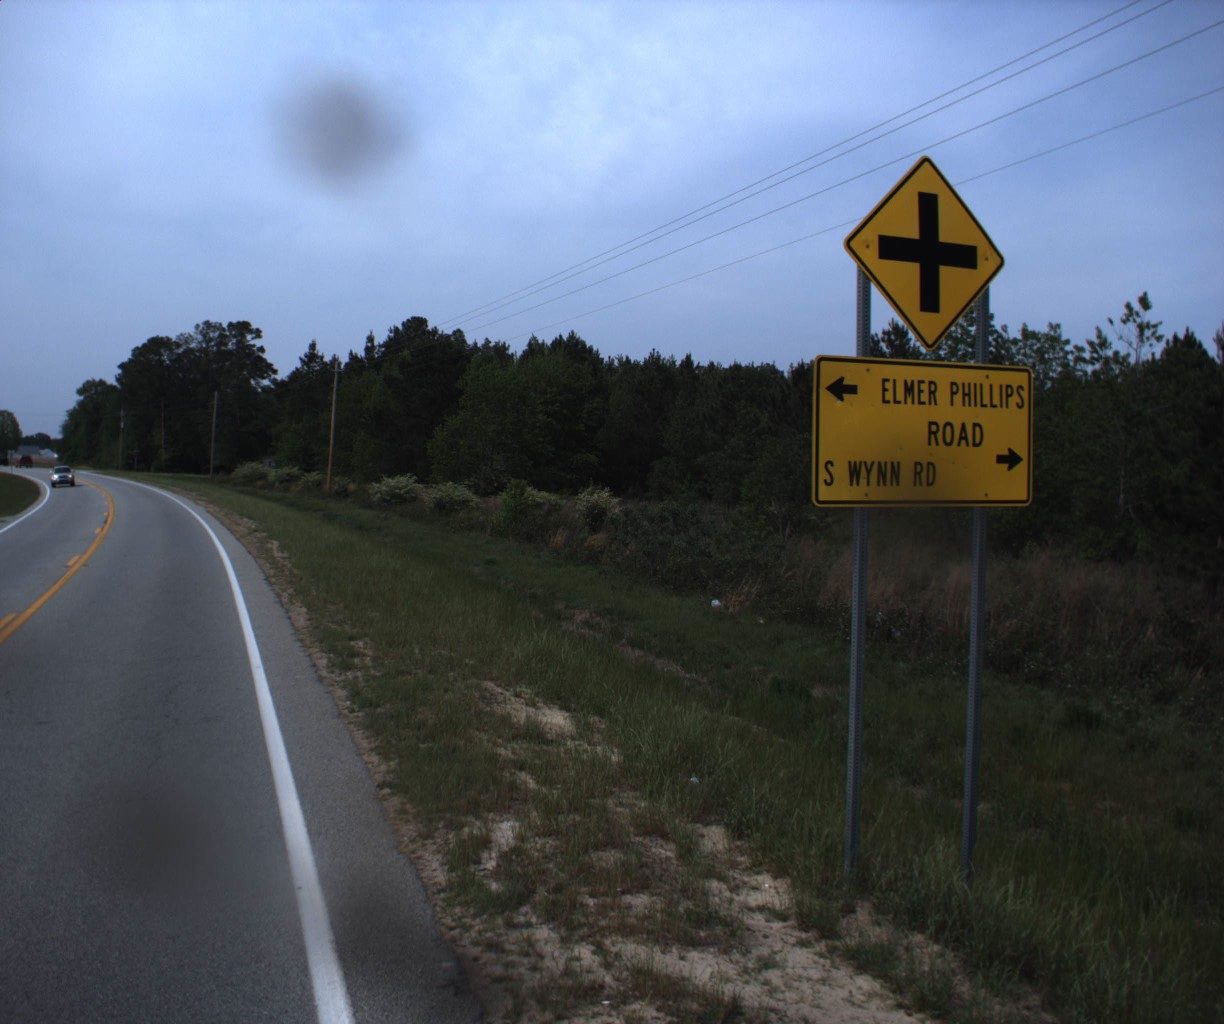
\includegraphics[width=13.333333333333334cm,height=7.333333333333333cm]{/home/nicolas/Programation/keras-cv/data/test/test.jpg}};

\pic[shift={ (2.3333333333333335,0,0) }] at (input) 
    {Box={
        name=Conv1-stride,
        caption= ,
        fill=\PoolColor,
        opacity=0.5,
        height=37.0,
        width=1,
        depth=67.0
        }
    };

\pic[shift={(0,0,0)}] at (Conv1-stride-east) 
    {Box={
        name=Conv1,
        caption= ,
        xlabel={{16, }},
        zlabel=100,
        fill=\ConvColor,
        height=18.333333333333332,
        width=4.0,
        depth=33.333333333333336
        }
    };

\pic[shift={(0,0,0)}] at (Conv1-east) 
    {Box={
        name=block_0_conv,
        caption= ,
        xlabel={{16, }},
        zlabel=100,
        fill=\ConvColor,
        height=18.333333333333332,
        width=4.0,
        depth=33.333333333333336
        }
    };

\pic[shift={ (2.3333333333333335,0,0) }] at (block_0_conv-east) 
    {Box={
        name=block_1_conv-stride,
        caption= ,
        fill=\PoolColor,
        opacity=0.5,
        height=18.333333333333332,
        width=1,
        depth=33.333333333333336
        }
    };

\draw [connection]  (block_0_conv-east)    -- node {\midarrow} (block_1_conv-stride-west);

\pic[shift={(0,0,0)}] at (block_1_conv-stride-east) 
    {Box={
        name=block_1_conv,
        caption= ,
        xlabel={{24, }},
        zlabel=50,
        fill=\ConvColor,
        height=9.333333333333334,
        width=4.584962500721157,
        depth=16.666666666666668
        }
    };

\pic[shift={(0,0,0)}] at (block_1_conv-east) 
    {Box={
        name=block_2_conv,
        caption= ,
        xlabel={{24, }},
        zlabel=50,
        fill=\ConvColor,
        height=9.333333333333334,
        width=4.584962500721157,
        depth=16.666666666666668
        }
    };

\pic[shift={(0,0,0)}] at (block_2_conv-east) 
    {Box={
        name=block_3_conv,
        caption= ,
        xlabel={{24, }},
        zlabel=50,
        fill=\ConvColor,
        height=9.333333333333334,
        width=4.584962500721157,
        depth=16.666666666666668
        }
    };

\pic[shift={ (2.3333333333333335,0,0) }] at (block_3_conv-east) 
    {Box={
        name=block_4_conv-stride,
        caption= ,
        fill=\PoolColor,
        opacity=0.5,
        height=9.333333333333334,
        width=1,
        depth=16.666666666666668
        }
    };

\draw [connection]  (block_3_conv-east)    -- node {\midarrow} (block_4_conv-stride-west);

\pic[shift={(0,0,0)}] at (block_4_conv-stride-east) 
    {Box={
        name=block_4_conv,
        caption= ,
        xlabel={{24, }},
        zlabel=25,
        fill=\ConvColor,
        height=4.666666666666667,
        width=4.584962500721157,
        depth=8.333333333333334
        }
    };

\pic[shift={(0,0,0)}] at (block_4_conv-east) 
    {Box={
        name=block_5_conv,
        caption= ,
        xlabel={{24, }},
        zlabel=25,
        fill=\ConvColor,
        height=4.666666666666667,
        width=4.584962500721157,
        depth=8.333333333333334
        }
    };

\pic[shift={(0,0,0)}] at (block_5_conv-east) 
    {Box={
        name=block_6_conv,
        caption= ,
        xlabel={{24, }},
        zlabel=25,
        fill=\ConvColor,
        height=4.666666666666667,
        width=4.584962500721157,
        depth=8.333333333333334
        }
    };

\pic[shift={(2.3333333333333335,3.3333333333333335,-2.0)}] at (block_3_conv-east) 
    {Box={
        name=output_1,
        caption= ,
        xlabel={{2, }},
        zlabel=50,
        fill=\ConvColor,
        height=9.333333333333334,
        width=1.0,
        depth=16.666666666666668
        }
    };

\draw [connection]  (block_3_conv-east)    -- node {\midarrow} (output_1-west);

\pic[shift={(2.3333333333333335,3.3333333333333335,2.0)}] at (block_3_conv-east) 
    {Box={
        name=output_2,
        caption= ,
        xlabel={{2, }},
        zlabel=50,
        fill=\ConvColor,
        height=9.333333333333334,
        width=1.0,
        depth=16.666666666666668
        }
    };

\draw [connection]  (block_3_conv-east)    -- node {\midarrow} (output_2-west);

\pic[shift={(2.3333333333333335,3.3333333333333335,-2.6666666666666665)}] at (block_6_conv-east) 
    {Box={
        name=output_3,
        caption= ,
        xlabel={{2, }},
        zlabel=25,
        fill=\ConvColor,
        height=4.666666666666667,
        width=1.0,
        depth=8.333333333333334
        }
    };

\draw [connection]  (block_6_conv-east)    -- node {\midarrow} (output_3-west);

\pic[shift={(2.3333333333333335,3.3333333333333335,0.0)}] at (block_6_conv-east) 
    {Box={
        name=output_4,
        caption= ,
        xlabel={{2, }},
        zlabel=25,
        fill=\ConvColor,
        height=4.666666666666667,
        width=1.0,
        depth=8.333333333333334
        }
    };

\draw [connection]  (block_6_conv-east)    -- node {\midarrow} (output_4-west);

\pic[shift={(2.3333333333333335,3.3333333333333335,2.6666666666666665)}] at (block_6_conv-east) 
    {Box={
        name=output_5,
        caption= ,
        xlabel={{2, }},
        zlabel=25,
        fill=\ConvColor,
        height=4.666666666666667,
        width=1.0,
        depth=8.333333333333334
        }
    };

\draw [connection]  (block_6_conv-east)    -- node {\midarrow} (output_5-west);

\end{tikzpicture}
\end{document}
